\documentclass[20pt, a1paper]{tikzposter}
\usepackage[utf8]{inputenc}

\usepackage{pgfpages}
%\pgfpagesuselayout{resize to}[a2paper]

\usepackage{graphicx}
\usepackage{wrapfig}
\usepackage{authblk}

\usepackage[backend=bibtex]{biblatex}
%\addbibresource{references.bib}

\title{Chat Application}

\author{Nils Jung}
\author{Jule Martensen}
\author{Marc Engelmann}
\author{Jan Steeg}

\affil{University of Applied Sciences Kiel}
\date{\today}

\usepackage{blindtext}
\usepackage{comment}

\usepackage{tikz}

\usetheme{Simple}

\makeatletter
\def\maketitle{\AB@maketitle}
\makeatother
\begin{document}
	\maketitle
	
	\begin{columns}
		\column{0.5}
	\block{Requirements \& Goal}
	{
		This accompanying JavaScript-based project has been realized as part of the mandatory course \textbf{Advanced Software Programming}.\\
		General requirements were:\\
	
		\begin{minipage}{0.55\linewidth}
			\begin{itemize}
				\item \textbf{Git} as version control service
				\item User sign-up and \textbf{authentication}
				\item \textbf{Database} access
				\item \textbf{Websockets}\\
			\end{itemize}
		\end{minipage}
		\begin{minipage}{0.45\linewidth}
		 \begin{tikzfigure}
		 	\includegraphics[width=0.75\textwidth]{../fullstack.png}
		 \end{tikzfigure}
		\end{minipage}
	\vspace{1.5cm}
		
		The goal behind these requirements is to reach abilities of \textbf{full stack}-development across modern web technologies throughout frontend and backend.\\
	}
	\block{Technologies}
	{
		\begin{itemize}
			\item \textbf{Frontend} (ReactJS, Redux, Bootstrap)
			\item \textbf{Backend} (NodeJS, Express, MongoDB)
			\item \textbf{Websockets} (Socket.IO)
			\item \textbf{Deployment} (Docker and Docker-Compose)
		\end{itemize}
		
		\begin{tikzfigure}
			\includegraphics[width=0.35\textwidth]{../techs.png}
		\end{tikzfigure}
	}
	\block{References}
	{
		\url{https://github.com/nilsjung/chat-application}\\
		\url{https://reactjs.org/}\\
		\url{https://redux.js.org/}\\

		\url{https://socket.io/}\\
		\url{https://getbootstrap.com/}\\
		\url{https://nodejs.org/}\\
		\url{https://expressjs.com/}\\
		\url{https://www.mongodb.com/}\\
	}

	\column{0.5}
	\block{Project idea}
	{
		The general idea was to develop a Chat Application on modern web technologies and frameworks with iterative integration (sprints) of new features such as:
		\begin{itemize}
			\item \textbf{in-chat-translation}
			\item \textbf{Emoji's}
			\item \textbf{Markdown} support
			\item \textbf{Recommendation of chatrooms} specific to user preferences
		\end{itemize}
	
	}
	\block{Features}
	{
		The following features based on user stories had been implemented during the semester:
		\begin{itemize}
			\item Fundamental chat functionality
			\begin{itemize}
				\item user registration \& authentication
				\item chat room communication
			\end{itemize}
			\item Translation of messages
			\item Emoji's 
		\end{itemize}
		
		\begin{minipage}[t][6cm]{0.5\linewidth}
			\begin{tikzfigure}
				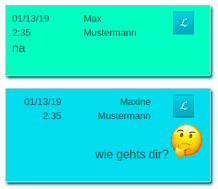
\includegraphics[scale=1.3]{chat-single.png}
			\end{tikzfigure}
		\end{minipage}		
		\begin{minipage}[t][6cm]{0.5\linewidth}
			\begin{tikzfigure}
				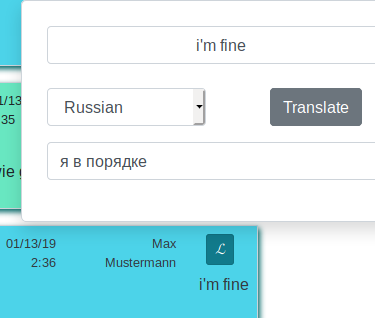
\includegraphics[scale=0.9]{chat-translation.png}
			\end{tikzfigure}
		
		\end{minipage}
		\vspace{3cm}
	}

	\block{Learnings}
	{
		\begin{itemize}
			\item Modern web development with focus on ReactJS and Redux
			\item Real-time communcation with Socket.IO
			\item Importance of Code Review
			\item Estimation of time for training of new technologies and development setup
			\item Experiments and training with new and unknown technologies / frameworks
			\item Docker as deployment technology
			\item Cooperation with gitflow workflow
		\end{itemize}
	}

	\end{columns}

	

	
\end{document}